En el presente proyecto se plantea desarrollar una aplicación de Aprendizaje de Máquina Supervisado de escritorio para el sistema operativo Windows 10 x64 en el transcurso de 8 meses a partir de Agosto del 2020. Esta aplicación tiene como finalidad permitir a estudiantes en su primeros años de formación académica en carreras como Ingeniería de Software, Sistemas, Informática y Computación, la selección del modelo, hiperparámetros, entrenamiento y predicción con base al conjunto de datos suministrado, por medio de una interfaz de usuario sencilla de comprender y documentación detallada de las funciones incorporadas.

\subsection{Etapas del proyecto}

Para cumplir los objetivos, la metodología de desarrollo ágil seleccionada para el proyecto es Scrumban, y además se tiene en cuenta las siguientes etapas: Inicio de proyecto, Diseño y planificación, Código e implementación, Evaluación y pruebas, y por último Conclusión del proyecto.

\subsubsection{Inicio de proyecto}
La primera etapa para el desarrollo del proyecto. Está compuesta de cinco actividades relacionadas al levantamiento de requerimientos y definición del alcance. Estas actividades tienen un componente directamente relacionado con reuniones de equipo y validación. Las actividades son:

\begin{APAitemize}
    \item Actividad 1. Reunión inicial de requerimientos: esta actividad consiste en la ejecución de la primera reunión del equipo, utilizando Zoom como medio para reunir a los integrantes de forma virtual, debido a la situación global del año 2020.
    \item Activad 2. Planteamiento de la metodología: a partir de las metodologías de desarrollo ágil existentes y las necesidades establecidas con anterioridad se define la metodología a trabajar utilizando reuniones de equipo. Esta actividad es paralela a la reunión inicial de requerimientos y se extiende hasta la validación de los requerimientos al final de la etapa.
    \item Actividad 3. Definición de tecnologías, lenguajes y \textit{frameworks}: teniendo en cuenta los requerimientos de la aplicación que se va a construir, se establecen el lenguaje de programación, los entornos de desarrollo, librerías, \textit{plugins} y \textit{frameworks}, de acuerdo a los conocimientos de los integrantes y de búsquedas en la web para posibles soluciones al problema planteado.
    \item Actividad 4. Validación de requerimientos establecidos: validar con todo el equipo a través de reuniones virtuales los requerimientos, metodología, tecnologías, lenguajes y \textit{frameworks} que se utilizaran a lo largo del desarrollo del proyecto.
    \item Actividad 5. Creación del reporte de requerimientos: creación y firma del reporte basado en una versión simplificada de la norma técnica colombiana para requerimientos de software. 
\end{APAitemize}

\subsubsection{Diseño y planificación}
Esta etapa está conformada por siete actividades relacionadas a la planeación, el diseño, documentación y validación. Por otro lado, esta etapa es la de mayor duración a comparación de las demás, por lo que un treinta por ciento del tiempo se distribuye para las actividades de diseño y planificación. Lo anteriormente mencionado se realiza a partir de las siguientes actividades:

\begin{APAitemize}
    \item Actividad 6. Planteamiento del cronograma: con base a los requerimientos, así como todas las funcionalidades del software, se establece el cronograma de actividades para un periodo de 8 meses a partir de Agosto del 2020.
    \item Actividad 7. Construcción del primer borrador: elaboración del primer \textit{wireframe}, así como el flujo de la aplicación entre cada formulario o vista. Este borrador a diferencia de un \textit{Mockup} no es diseñado en herramientas de prototipado como Figma, sino que es un boceto creado a mano.
    \item Actividad 8. Diseño de interfaz preliminar: primer diseño de la interfaz de usuario creada en Figma, teniendo en cuenta la ISO 11581-10:2010, 9241-112:2019 e 9241-210:2019 para la creación de interfaces de usuario. Este diseño se validada constantemente durante su desarrollo hasta su posterior aceptación como interfaz final, ya que no se debe regresar a etapas anteriores una vez se avance lo suficiente en el desarrollo de la aplicación.
    \item Actividad 9. Validación de interfaz de usuario: a través de reuniones de equipo en Zoom, se aprueba el diseño presentado como la interfaz final para posterior implementación e integración con el código fuente.
    \item Actividad 10. Diseño del \textit{back-end}: teniendo en cuenta las entradas y salidas de la aplicación, al igual que el diseño de interfaz de usuario aceptada hasta el momento, se diseña el código fuente del \textit{back-end} utilizando diagramas UML de clase, así como patrones de diseño para su creación.
    \item Actividad 11. Validación final del diseño: una vez terminadas las actividades relacionadas al diseño, se realiza la validación final para su posterior puesta en producción por parte del equipo de trabajo a través de reuniones en Zoom. La evidencia de esas reuniones se encuentran como capturas de pantalla en el repositorio del proyecto.
    \item Actividad 12. Construcción del reporte de diseño: con base a los diagramas UML de casos de uso y clase, así como la documentación generada a partir de los documentos creados a partir de la norma técnica colombiana simplificada, se genera y valida el reporte con los documentos anteriormente mencionados.
\end{APAitemize}

\subsubsection{Código e implementación}
Esta etapa consiste en cinco actividades, siendo estas en su mayoría la creación de código fuente, tanto para el \textit{front-end} como para el \textit{back-end}. Aun así, en esta etapa se realizan labores de documentación y revisiones de código, con el fin de producir software de calidad. Por último, esta etapa que tiene una duración menor al diseño y se conforma de las siguientes actividades:

\begin{APAitemize}
    \item Actividad 13. Construcción de pruebas y código fuente: a partir del diseño previamente establecido, se genera el código fuente de la aplicación al mismo tiempo que se crean pruebas de validación e integración para su posterior ejecución. Este código debe de seguir los estándares PEP8, PEP20, PEP257, PEP3131, PEP 484 y PEP 526 para Python, el cual es el principal lenguaje que se utiliza en el proyecto.
    \item Actividad 14. Construcción de la interfaz de usuario: a partir del \textit{wireframe} y mockup previamente desarrollados se crea la interfaz en QT Designer para su posterior implementación en la aplicación.
    \item Actividad 15. Revisión del código desarrollado: por medio de revisiones con el equipo utilizando Zoom y las herramientas proporcionadas en GitHub, se analiza línea a línea el código generado con el fin de evitar cambios y errores que no se encuentren a tiempo durante el desarrollo del proyecto.
    \item Actividad 16. Documentación del código fuente: después de realizarse las actividades relacionadas a la creación del código fuente y sus revisiones, se realiza la documentación detallada para cada función, método y clase, con el objetivo de presentar código fuente más legible y que además pueda ser entendido con mayor facilidad por los demás miembros del equipo.
    \item Actividad 17. Integración \textit{front-end} y \textit{back-end}: una vez terminado el desarrollo del código fuente tanto del \textit{front-end} como del \textit{back-end}, se realiza la integración de ambos en un solo ambiente. Adicionalmente se escriben pruebas de software relacionadas a la integración del sistema para garantizar el funcionamiento de la aplicación.
\end{APAitemize}

\subsubsection{Evaluación y pruebas}
En el transcurso de esta etapa la cual cuenta con cuatro actividades, se centran los esfuerzos del equipo en ejecutar pruebas de software, corregir los errores producto de la integración entre el \textit{front-end} y el \textit{back-end}, y finalmente documentar los resultados. Esta penúltima etapa del proyecto está conformada por las siguientes actividades:

\begin{APAitemize}
    \item Actividad 18. Ejecución pruebas de software: una vez integrado el sistema con su debida documentación, se ejecutan nuevamente todas las pruebas creadas hasta el momento, pero adicionalmente se realiza pruebas de regresión, así como pruebas de caja negra donde se pruebe la aplicación paso a paso por cada una de las rutas existentes.
    \item Actividad 19. Corrección de errores: esta actividad consiste en la corrección del código fuente con base a los resultados obtenidos en la ejecución de pruebas de software.
    \item Actividad 20. Validación de los cambios: a través de revisiones de código con el equipo, se revisan los cambios generados con base a los resultados de las pruebas de software. 
    \item Actividad 21. Documentación de las pruebas: de acuerdo al código generado en anteriores actividades y los resultados de las pruebas antes y después de correcciones, se genera la documentación de las pruebas a partir de una versión simplificada de la norma técnica colombiana para pruebas de software.
\end{APAitemize}

\subsubsection{Conclusión del proyecto}
La última etapa del presente proyecto se conforma de tres actividades que se desarrollaran en el último mes antes de cumplir con la fecha límite. Las actividades correspondientes a la conclusión del proyecto son:

\begin{APAitemize}
    \item Actividad 22. Validación final de funcionalidades: utilizando máquinas virtuales y equipos ajenos al desarrollo, la aplicación se pone bajo pruebas de usuario final para validar su correcto funcionamiento. En caso de existir errores inesperados se debe de volver a realizar la compilación del ejecutable con los cambios pertinentes, hasta que los inconvenientes sean menores a la cantidad mínima requerida para su validación final.
    \item Actividad 23. Creación del manual de usuario: considerando las funcionalidades de la aplicación, al igual que la rutas posibles que se ofrecen, se crea un manual de usuario que contenga la guía de instalación del software, los requerimientos mínimos del sistema y los procedimientos paso a paso para el uso correcto de la aplicación.
    \item Actividad 24. Despliegue de la aplicación: dada la completitud de todas las etapas y sus actividades, se libera la aplicación para el uso del público en el repositorio de GitHub bajo la licencia BSD 3. Adicionalmente, se entrega la documentación generada, el código fuente y el instalador de la aplicación a la institución de educación superior donde se desarrolla el proyecto.
\end{APAitemize}

\subsection{Descripción de la herramienta}

Voorspelling dispone de veintiséis vistas o páginas desarrolladas en QT Designer e implementadas con Python y el \textit{plugin} PyQt5. El flujo de la aplicación inicia con la vista de inicio y termina con los resultados paso a paso o automáticos de acuerdo a la ruta seleccionada, así como muestra la figura \ref{fig:workflow}. Sin embargo, el flujo normal de la aplicación al seleccionar aprendizaje automático solo necesita cinco vistas, mientras que la opción de aprendizaje paso a paso puede variar entre diez y once, de las cuales una de estas tiene doce diferentes formas de presentarse si el usuario requiere seleccionar los hiperparámetros bajo su criterio.

\begin{figure}[H]
    \centering
    \caption{Flujo de la aplicación}
    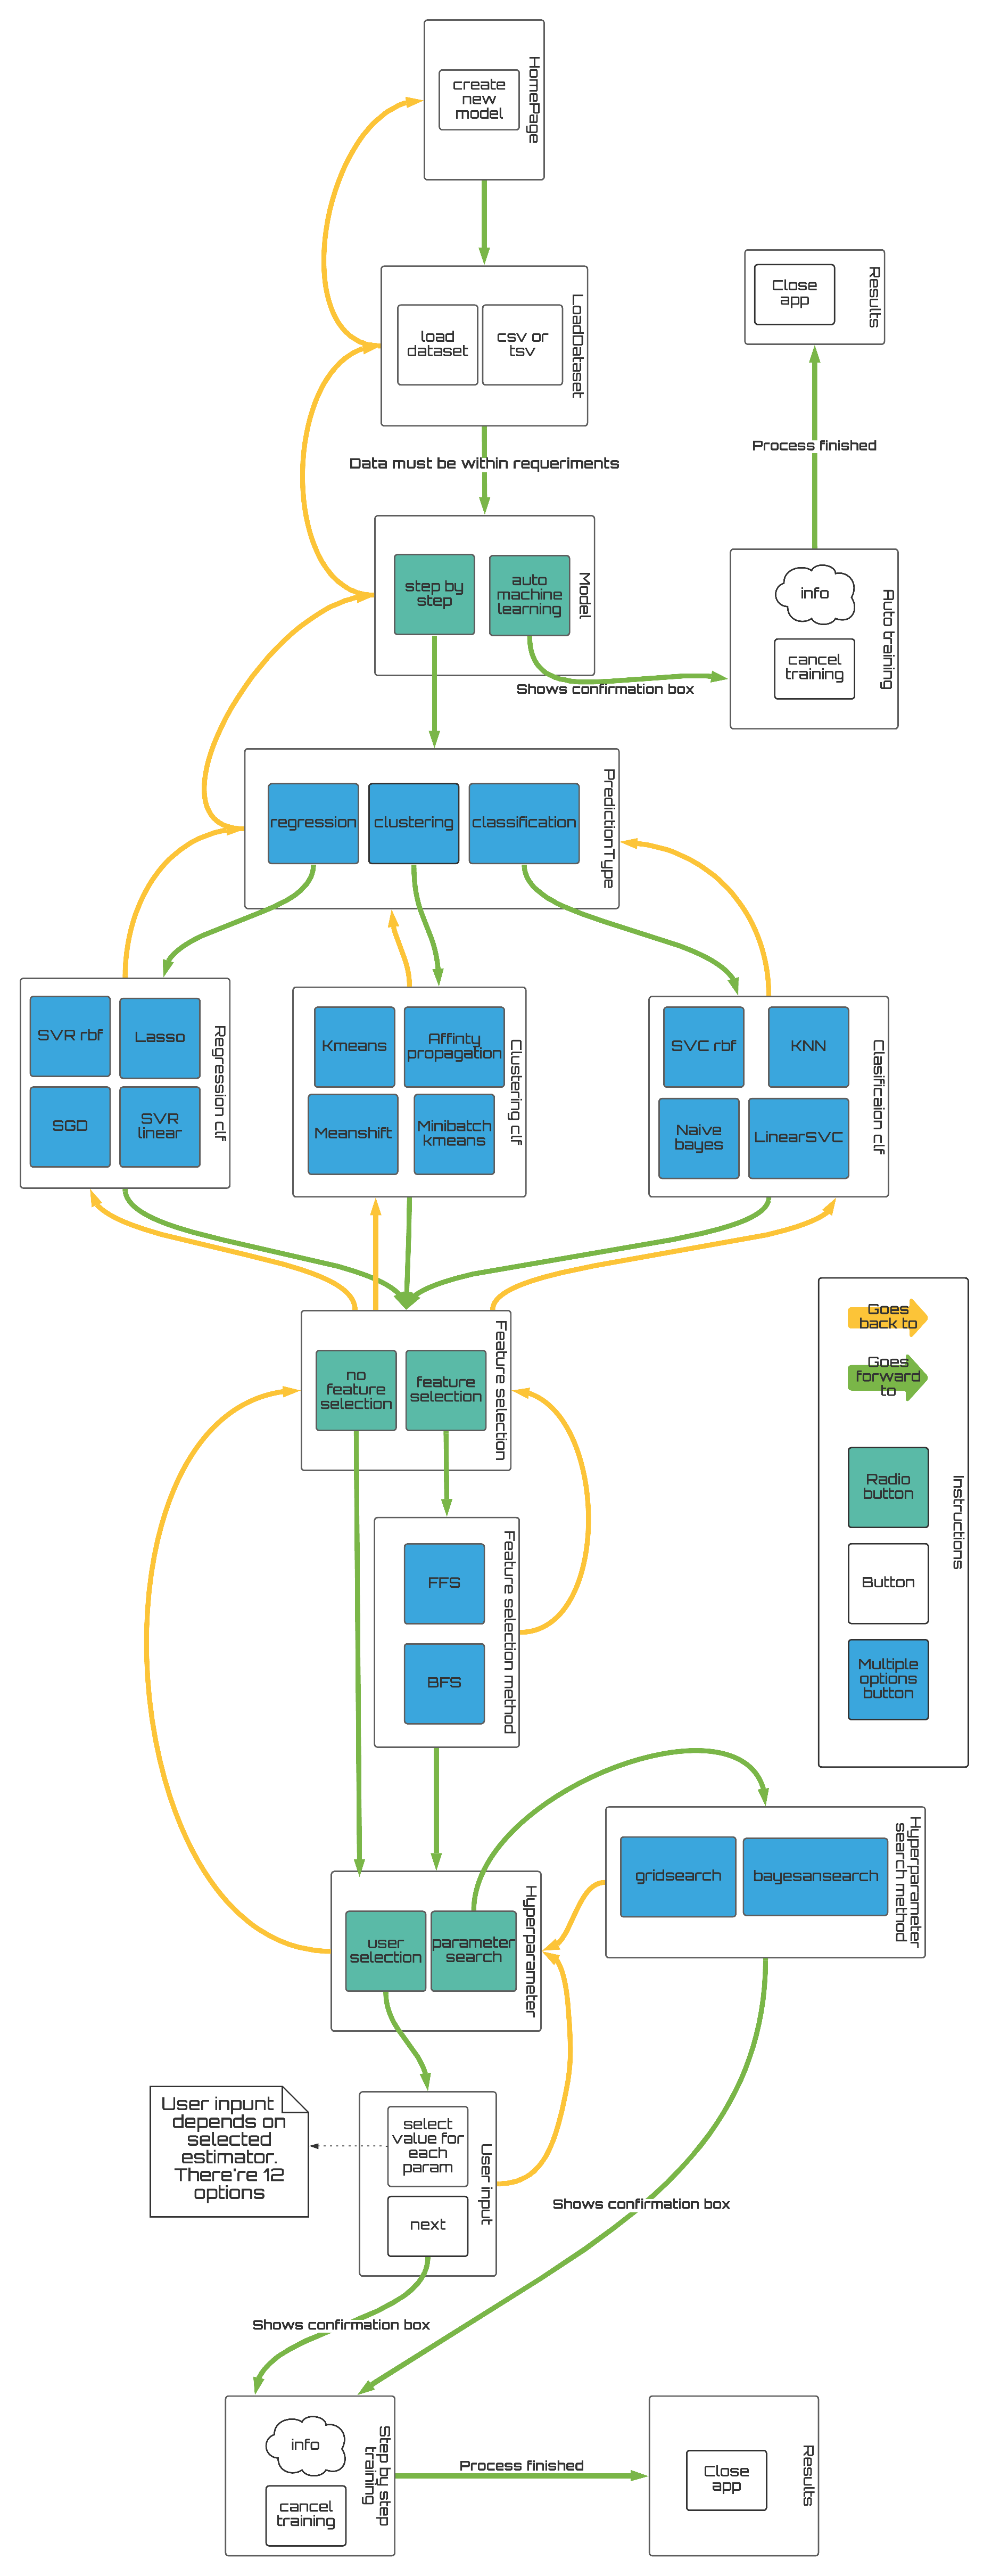
\includegraphics[width=\textwidth, height=\textheight,keepaspectratio]{images/appworkflow.png}
    \label{fig:workflow}
\end{figure}

La primera vista al igual que las demás presenta el titulo en la parte superior central, el icono en la parte superior izquierda, los datos del equipo de desarrollo en la parte lateral izquierda y otros datos como el nombre completo de la aplicación, año de creación e institución donde se desarrolla. Ver figura \ref{fig:home}.

\begin{figure}[H]
    \centering
    \caption{Página: inicio}
    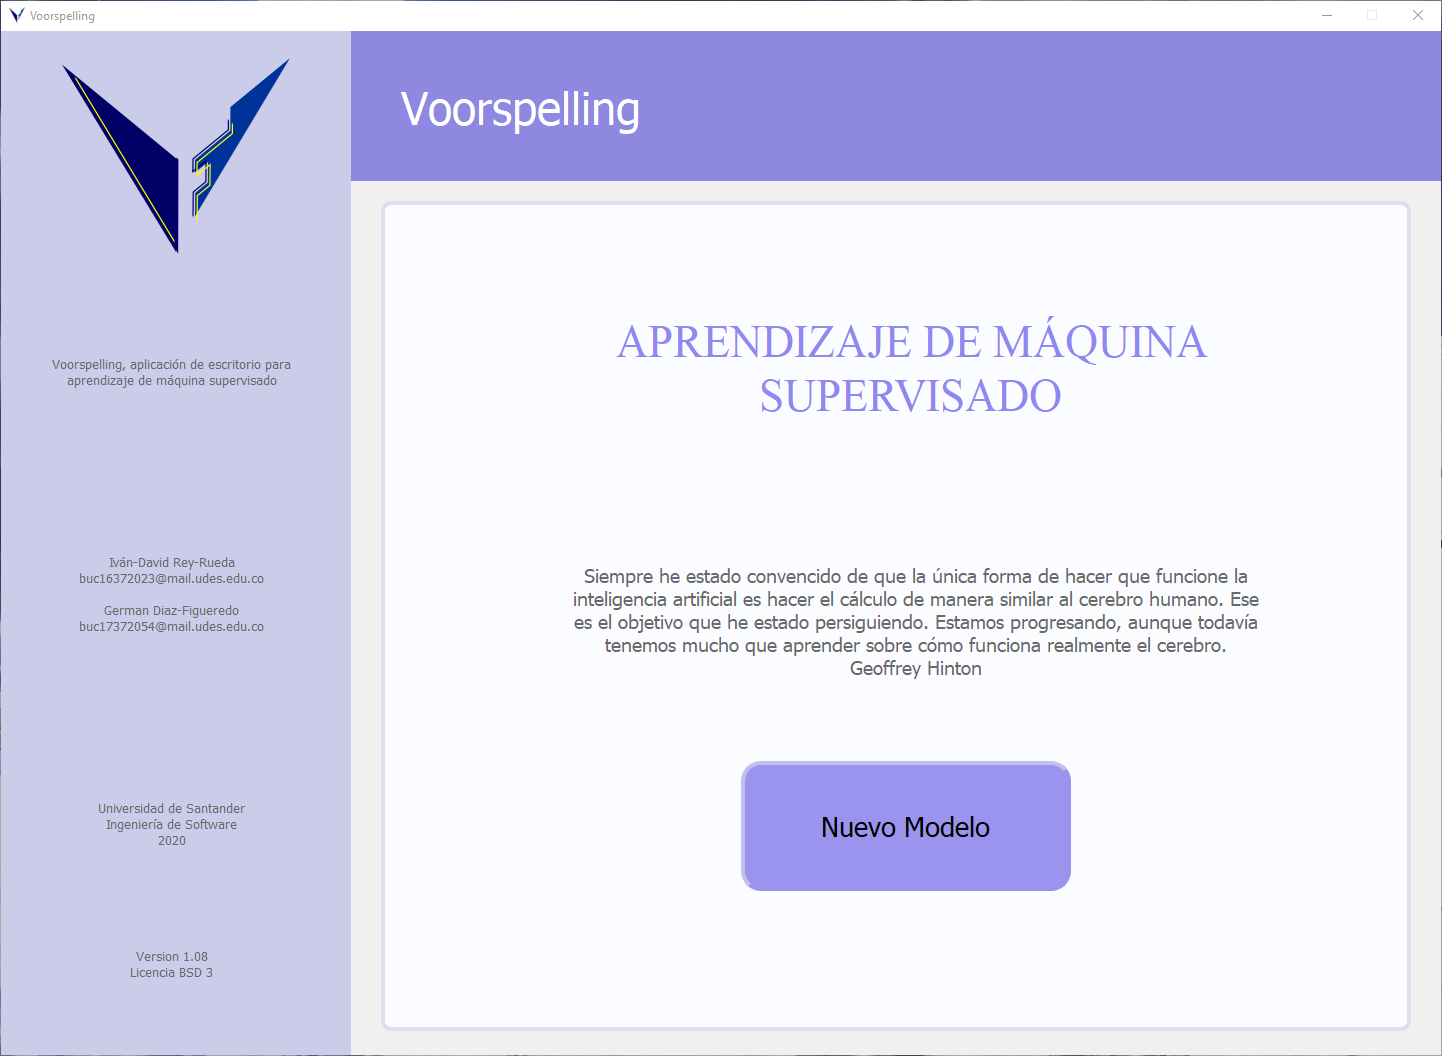
\includegraphics[width=\textwidth]{views/home.png}
    \label{fig:home}
\end{figure}

La aplicación cambia a la segunda vista cuando se presiona el botón \textit{nuevo modelo} desde la página de inicio. Como se muestra en la figura \ref{fig:loaddataset}, se presenta la opción de seleccionar entre \textit{TSV} y \textit{CSV}, subir o arrastrar un archivo, mirar información de ayuda, regresar a la vista anterior y finalmente continuar con el proceso al presionar el botón \textit{siguiente}.

\begin{figure}[H]
    \centering
    \caption{Página: cargar conjunto de datos}
    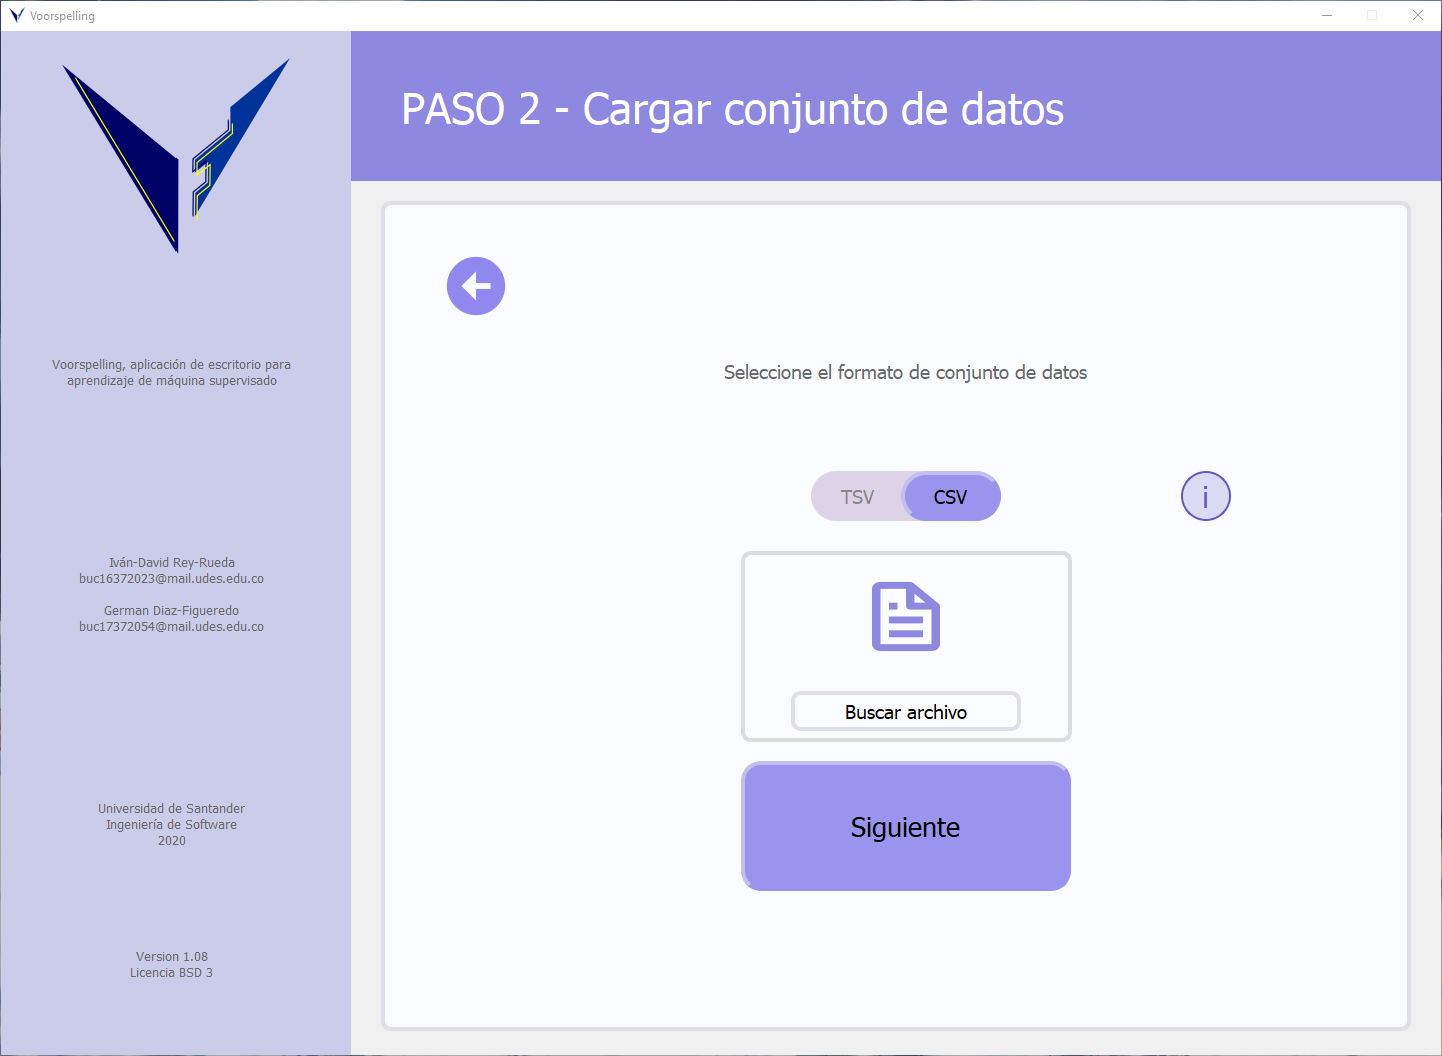
\includegraphics[width=\textwidth]{views/load_dataset.png}
    \label{fig:loaddataset}
\end{figure}

En la tercera vista como se muestra en la figura \ref{fig:modeltype}, el usuario puede seleccionar entre las dos opciones, mirar información de ayuda, regresar a la vista anterior y finalmente continuar con el proceso al presionar el botón \textit{siguiente}. Si la opción seleccionada es \textit{modelo de aprendizaje automático}, entonces la aplicación muestra una ventana emergente para confirmar la ruta seleccionada, mientras que por la otra ruta el programa redirige al usuario al paso cuatro.

\begin{figure}[H]
    \centering
    \caption{Página: tipo de modelo}
    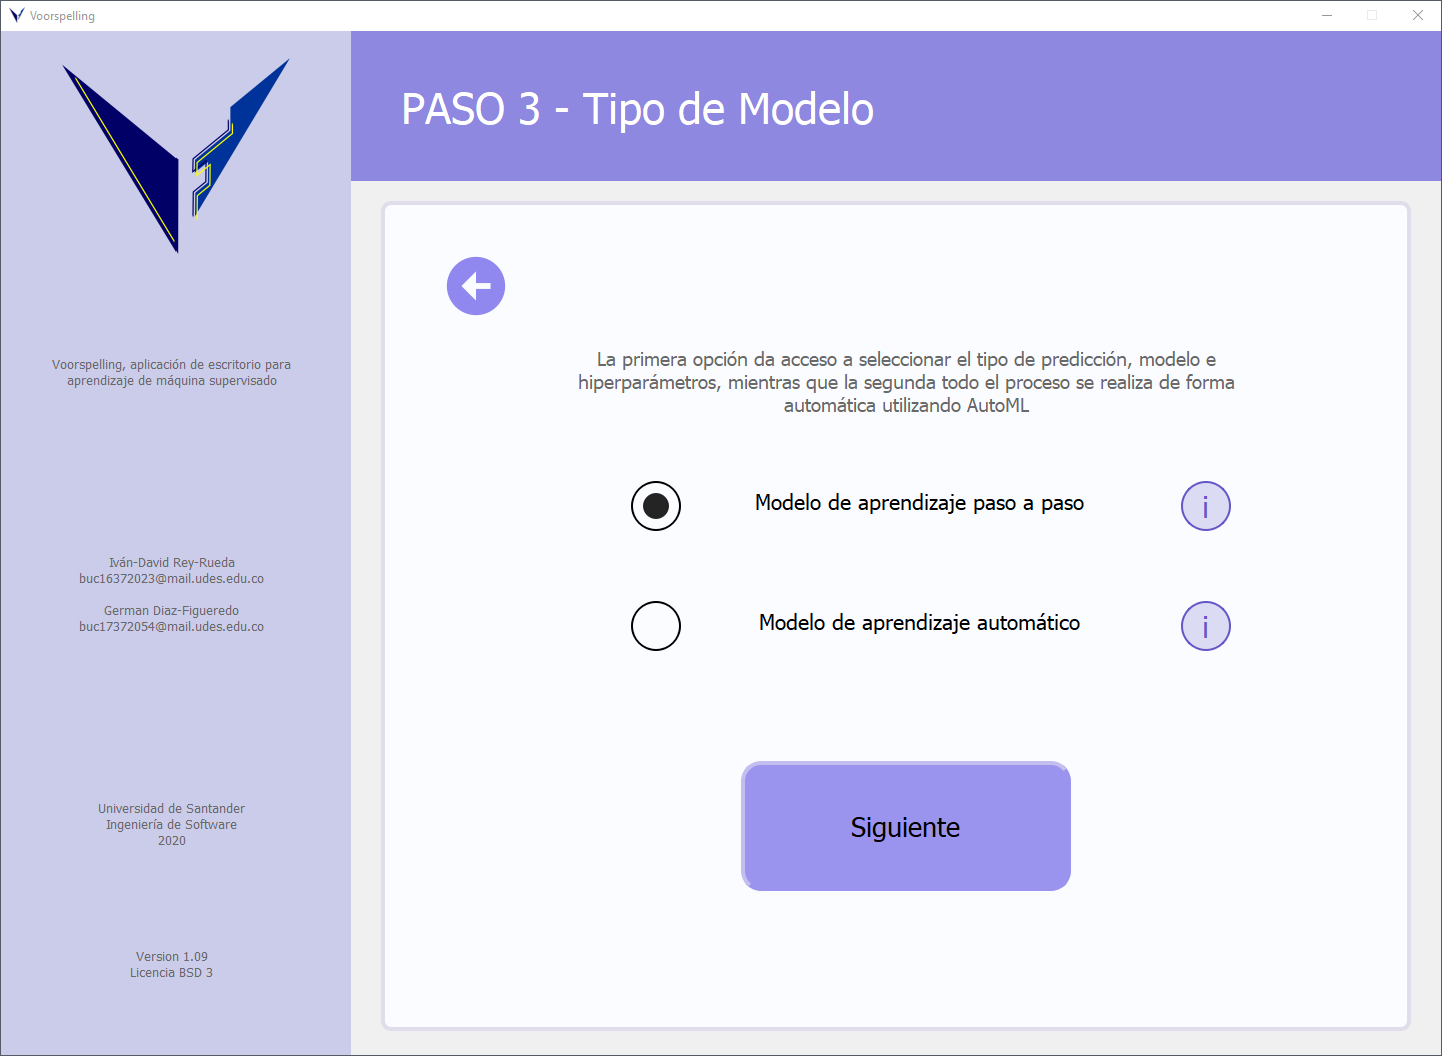
\includegraphics[width=\textwidth]{views/model.png}
    \label{fig:modeltype}
\end{figure}

\subsubsection{modelo automático}

Una vez iniciado el entrenamiento la aplicación muestra en pantalla información en tiempo real la información del modelo. El usuario puede optar por esperar a que el proceso finalice o presionar el botón \textit{cancelar entrenamiento} para detener el proceso en segundo plano (ver Figura \ref{fig:training}). La opción de interrumpir o no el entrenamiento se despliega en una ventana emergente, la cual informa al usuario de las consecuencias de realizar esa acción.

\begin{figure}[H]
    \centering
    \caption{Página: entrenamiento del modelo}
    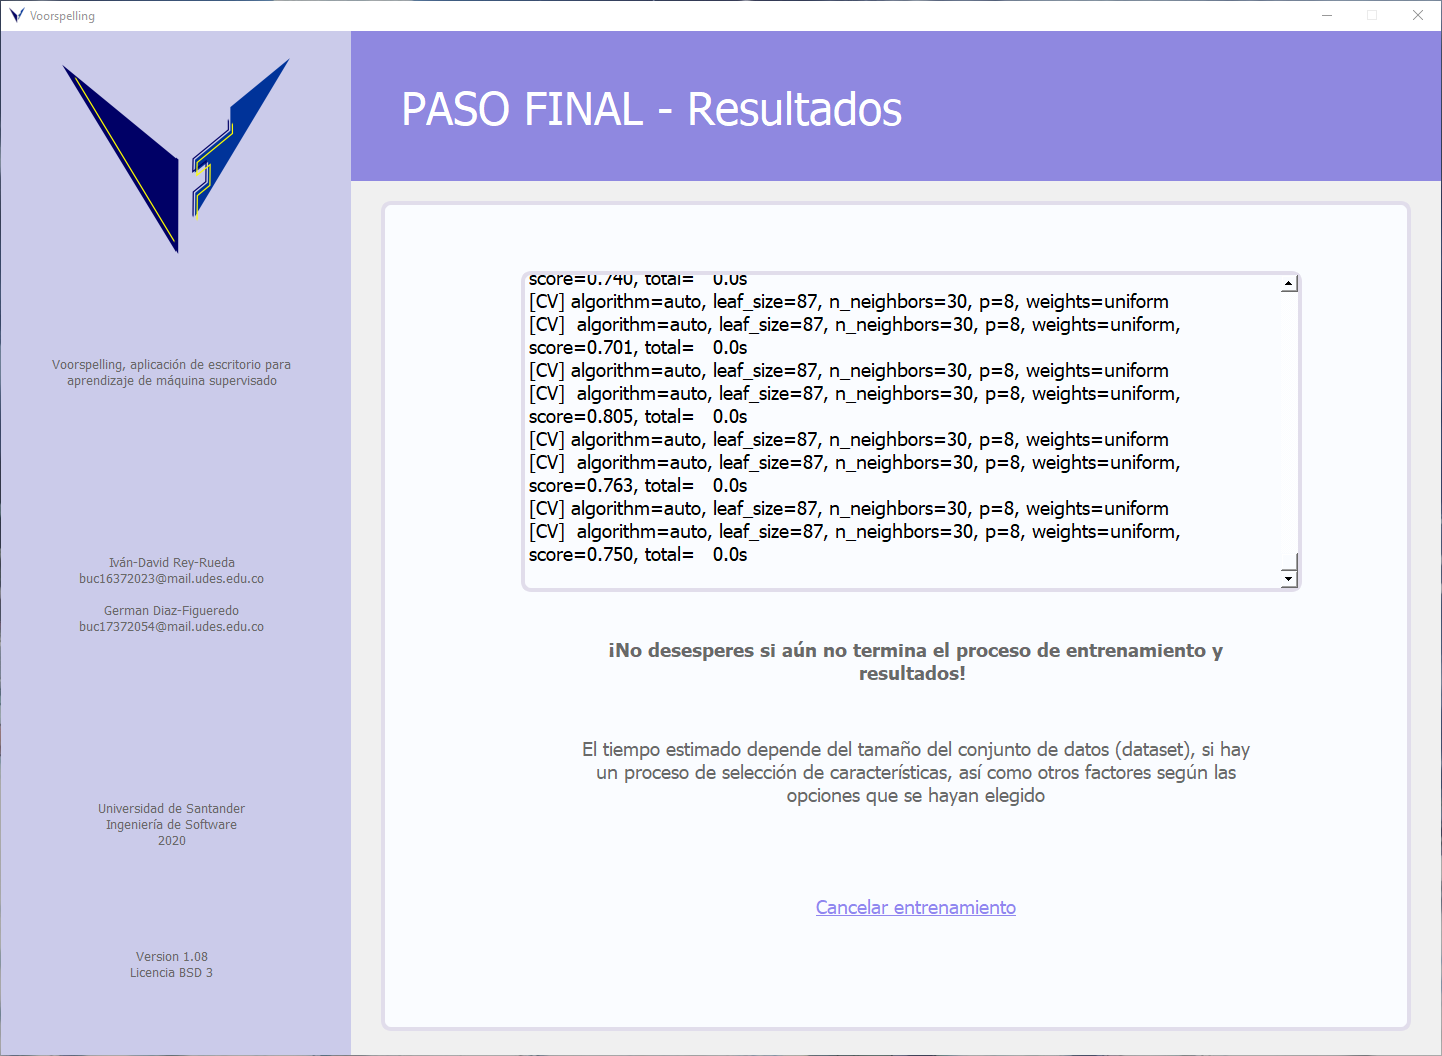
\includegraphics[width=\textwidth]{views/training.png}
    \label{fig:training}
\end{figure}

Si el proceso de entrenamiento termina exitosamente la aplicación redirige al usuario a la vista final donde se muestra la información final, los enlaces del repositorio de mljar-supervised y Voorspelling, aclaraciones de la carpeta de resultados y finalmente el botón \textit{finalizar} para cerrar la aplicación. Ver figura \ref{fig:trainingrslt}.

\begin{figure}[H]
    \centering
    \caption{Página: resultados del entrenamiento}
    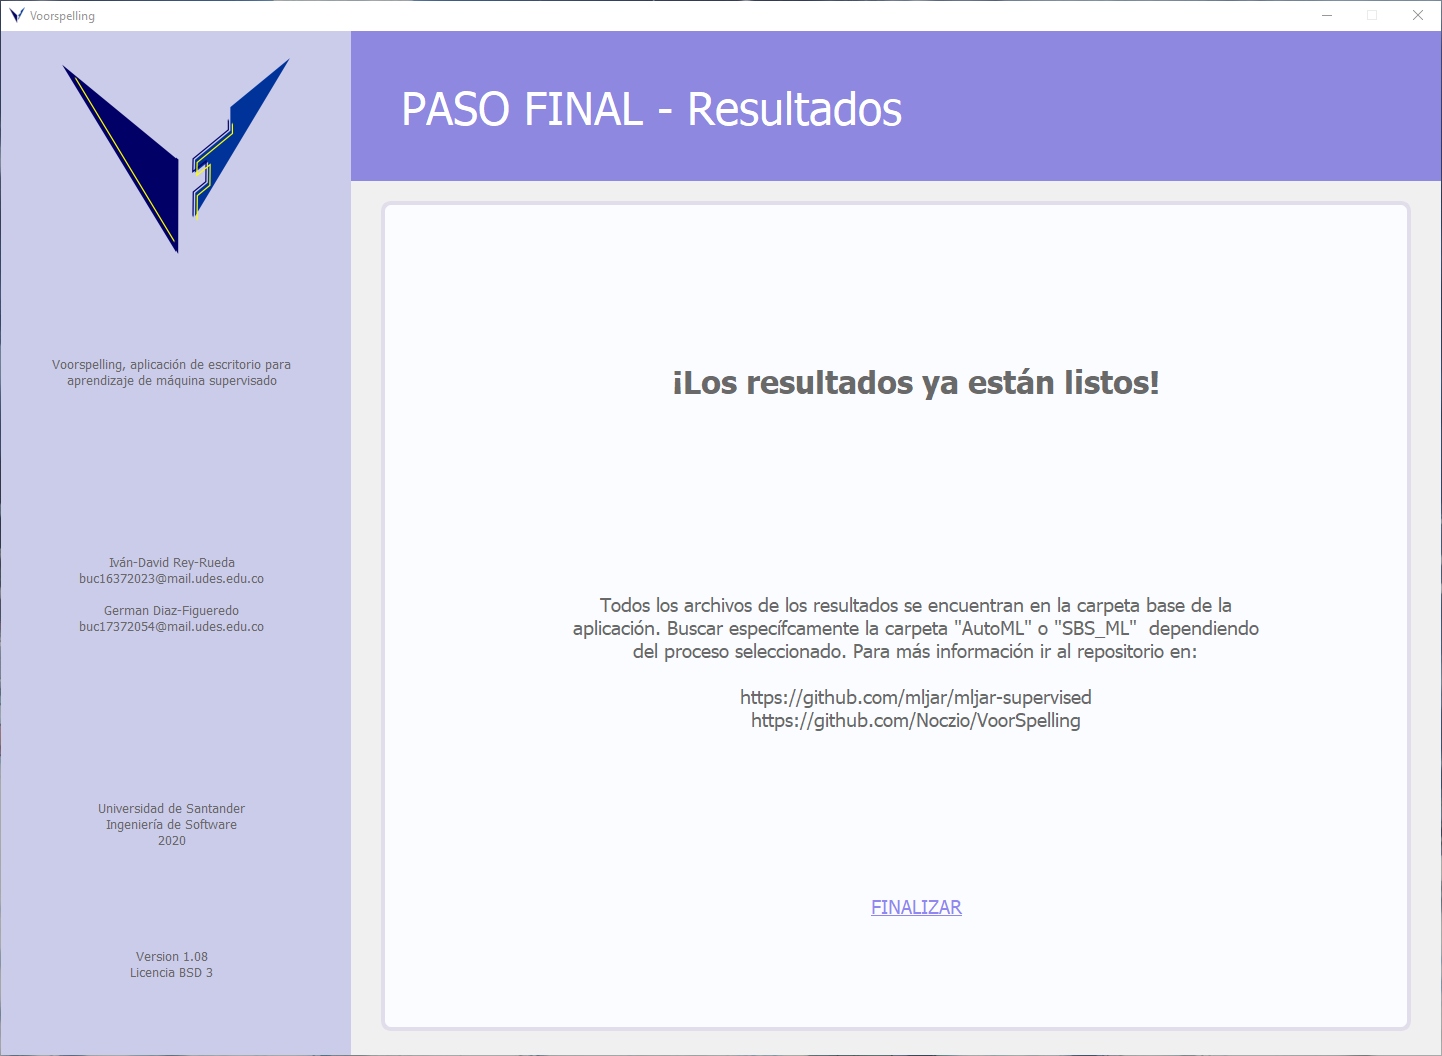
\includegraphics[width=\textwidth]{views/final.png}
    \label{fig:trainingrslt}
\end{figure}

Los resultados se encuentran guardados en la ruta de instalación de la aplicación, así como se menciona en la Figura \ref{fig:trainingrslt}. No obstante, el nombre de la carpeta varia de acuerdo al número de modelos entrenados, ya sean automáticos o paso a paso.

\subsubsection{modelo paso a paso}

Si en la vista de tipo de modelo se elige \textit{paso a paso}, la aplicación redirige al usuario a la selección del tipo de predicción, es decir, clasificación, regresión y agrupamiento. Esta página permite regresar a la vista anterior, ver información de ayuda y seleccionar el tipo de predicción con las tres opciones mencionadas anteriormente. Ver Figura \ref{fig:predictiontype}.

\begin{figure}[H]
    \centering
    \caption{Página: tipo de predicción}
    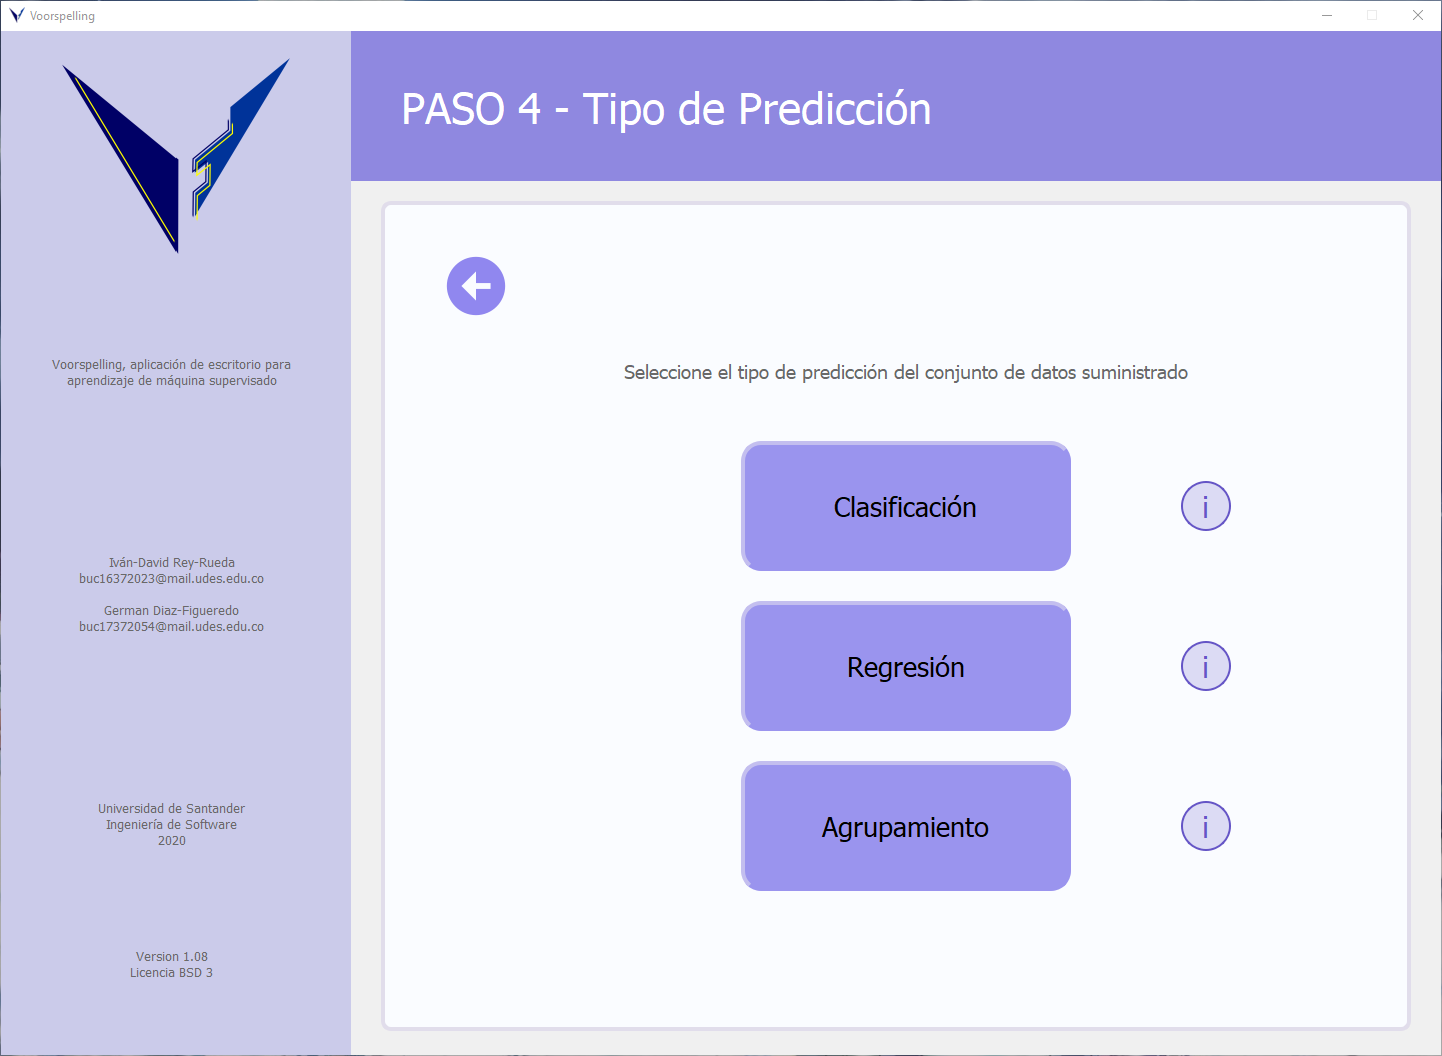
\includegraphics[width=\textwidth]{views/prediction_type.png}
    \label{fig:predictiontype}
\end{figure}

En dado caso de seleccionar \textit{clasificación} la aplicación cambia la vista a la mostrada en la Figura \ref{fig:classificationestimators}, mientras que al seleccionar \textit{regresión} se redirige al usuario a la vista de la Figura \ref{fig:regressionestimators} y finalmente seleccionar la opción \textit{agrupamiento} cambia la vista a la selección del estimador como muestra la Figura \ref{fig:clusterestimators}. Cada una de estas vistas tienen la opción de regresar al paso anterior y ver información de ayuda; al igual que cada página de Voorspelling.

Una vez los requerimientos para continuar se cumplen en las vistas para selección de estimador, la siguiente página que se despliega permite seleccionar si se requiere utilizar un proceso de selección de características (Ver Figura \ref{fig:wantfeatureselection}).

\begin{figure}[H]
    \centering
    \caption{Página: selección de características}
    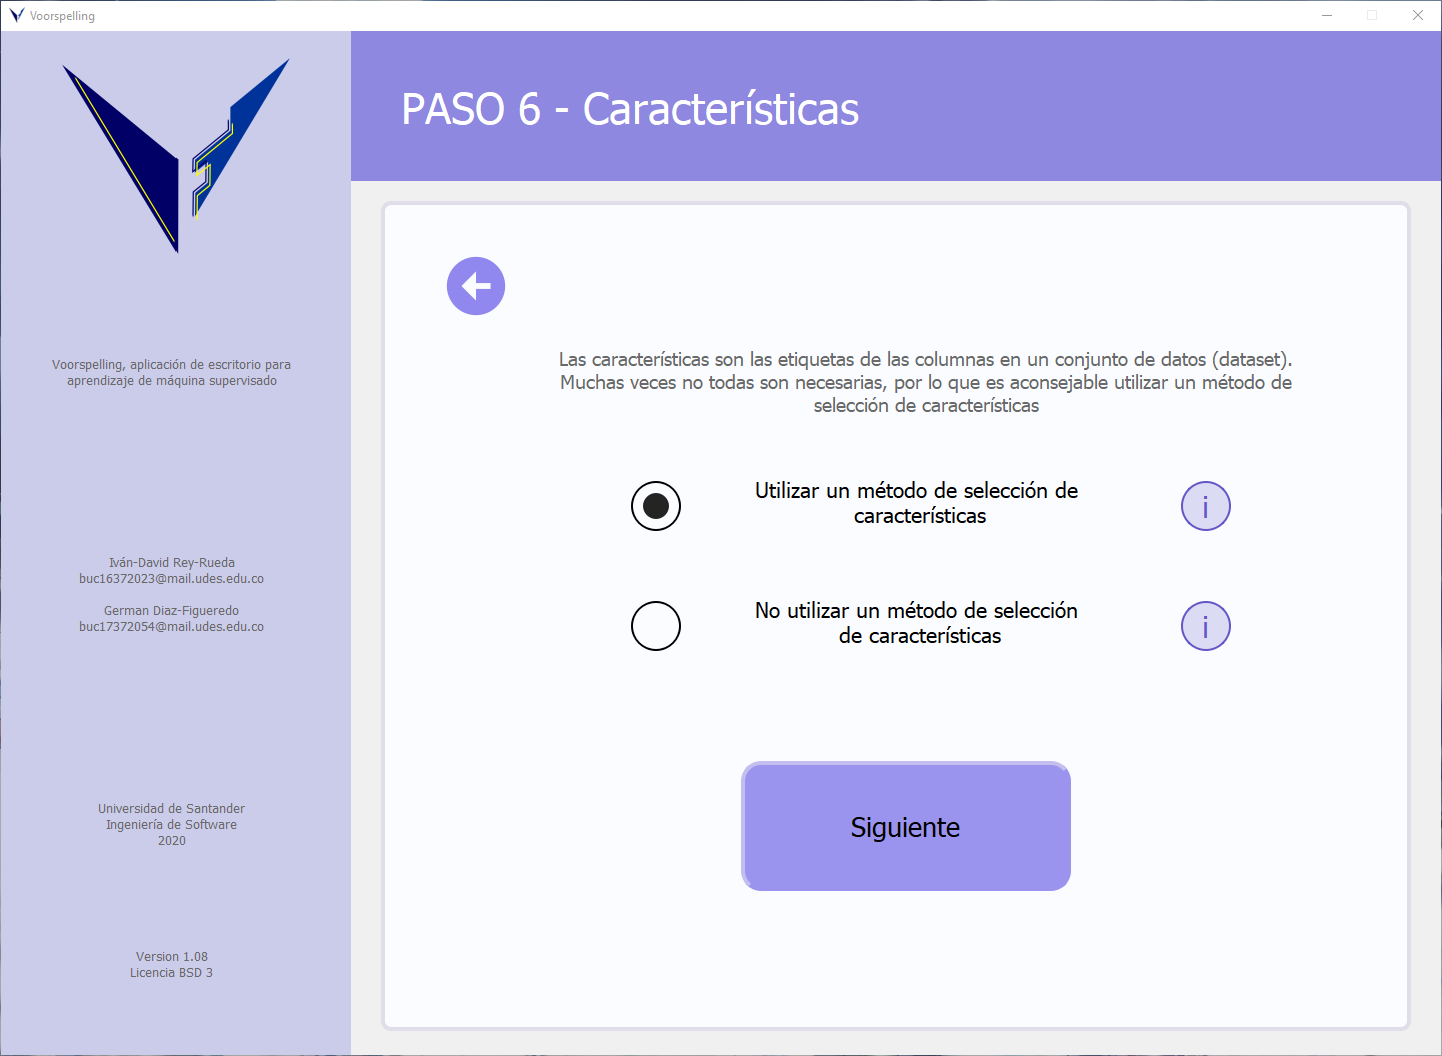
\includegraphics[width=\textwidth]{views/want_feature_selection.png}
    \label{fig:wantfeatureselection}
\end{figure}

Si se requiere de un proceso de selección de características la aplicación muestra la vista como se ve en la Figura \ref{fig:featureselectionmethod}, mientras que si no se necesita, inmediatamente se redirige al usuario al siguiente paso. Una ves cumplido los requerimientos para continuar, la siguiente página tiene el objetivo de seleccionar si se requiere de un proceso de búsqueda de hiperparámetros. Ver Figura \ref{fig:wanthiperparametersearch}.

\begin{figure}[H]
    \centering
    \caption{Página: búsqueda de hiperparámetros}
    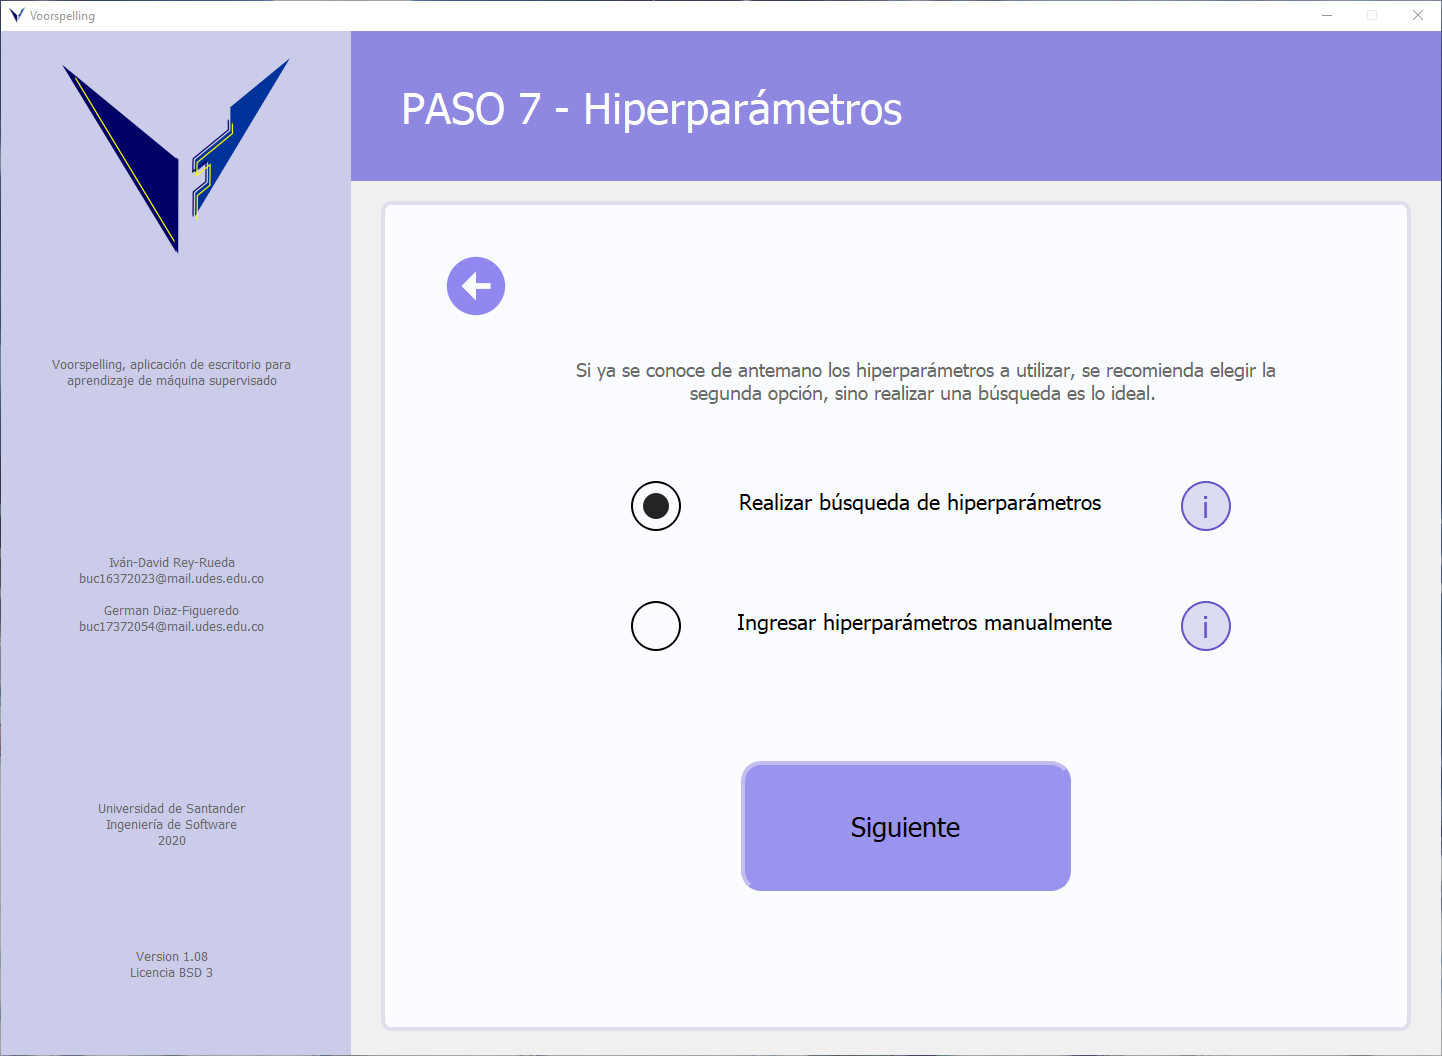
\includegraphics[width=\textwidth]{views/want_hiperparameter_search.png}
    \label{fig:wanthiperparametersearch}
\end{figure}

En dado caso si el usuario requiere de un proceso de búsqueda de hiperparámetros, la aplicación muestra la vista al igual como se muestra en la Figura \ref{fig:hiperparamsearchmethod}, mientras que si no se necesita, se redirige al usuario al siguiente paso donde se elige los hiperparámetros uno a uno dependiendo del estimador elegido. Finalmente una vez se cumplen los requerimientos para continuar al siguiente paso desde cualquier de las vistas posibles, ya sea con alguno de los métodos de búsqueda de hiperparámetros o si no se requiere (Ver Figuras \ref{fig:knn}, \ref{fig:knn}, \ref{fig:linearsvc}, \ref{fig:svc}, \ref{fig:gassianNB}, \ref{fig:lasso}, \ref{fig:linearsvr}, \ref{fig:svr}, \ref{fig:sgd}, \ref{fig:affinitypropagation}, \ref{fig:kmeans}, \ref{fig:minibatchkmeans} y \ref{fig:meanshift}), el proceso de entrenamiento inicia y sigue el mismo proceso descrito para un modelo automático (ver Figuras \ref{fig:training} y \ref{fig:trainingrslt}).
